\chapter{Omringende logica}
\label{periphery}

Een heleboel logische blokken, zoals decoders, drivers, pass-gates en buffers zitten verwerkt in de geheugenstructuur.
In dit hoofdstuk worden deze componenten van wat dichterbij onderzocht.

\section{Decoders}
Een decoder is een logische blok dat een uitgang selecteert op basis van een geencodeerde bus van ingangen. Aangezien het aantal globalblocks, woordlijnen en bitlijnen nog niet vastgelegd werd, werd er een gamma van decoders ontworpen gaande van een 2 naar 4 decoder tot en met een 9 naar 512 decoder. Voor het ontwerp van de grotere decoders, werd er gebruik gemaakt van de kleinere decoders als bouw blokken. Dit kan gedaan worden op 2 manieren; volgens een tree patroon (\ref{fig:decoder1}) of volgens een grid patroon (\ref{fig:decoder2}). In de volgende secties word het ontwerp van beide manieren toegelicht, en vergeleken.

\begin{figure}[!ht]
\centering
\subfloat[Decoder type 1]{ 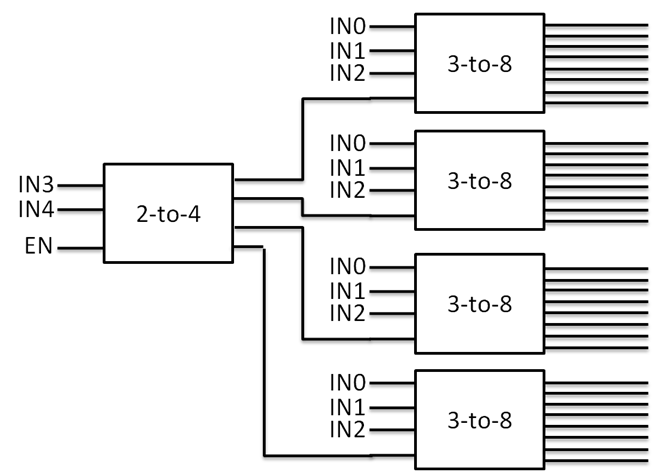
\includegraphics[width=0.45\textwidth] {../fig/hfdst-decoders-type1.png} \label{fig:decoder1}}
\subfloat[Decoder type 2]{ 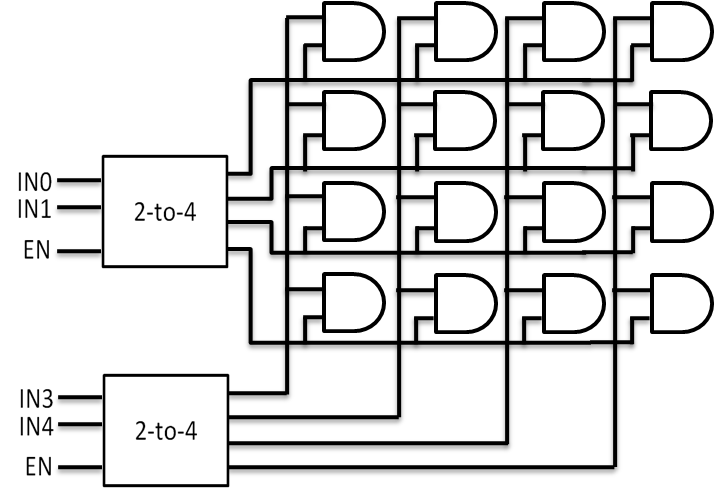
\includegraphics[width=0.45\textwidth] {../fig/hfdst-decoders-type2.png} \label{fig:decoder2}}
\caption{Opbouw voor grotere decoders}\label{fig:basisdecoders}
\end{figure}

\subsection{De tree decoder}
De tree decoder is een decoder met een meerlaagse structuur dat zich uitwaaiered naar de uitgangen. De basis blokken van deze decoder zijn een 2 naar 4 decoder (figuur \ref{fig:decoder2to4}) en een 3 naar 8 decoder (figuur \ref{fig:decoder3to8}). In elke laag in deze structuur komen een aantal ingangen binnen en deze gaan naar de ingang van evenveel decoders als er uitgang zijn in de vorige laag. Elke uitgange van de vorige laag stuurt de enble van een van de decoders van de huidige laag aan. Dit word geillustreed in de vorm van een 5 naar 32 decoder in figuur \ref{fig:decoder1}. 
\begin{figure}[!ht]
\centering
\subfloat[2 naar 4 decoder]{ 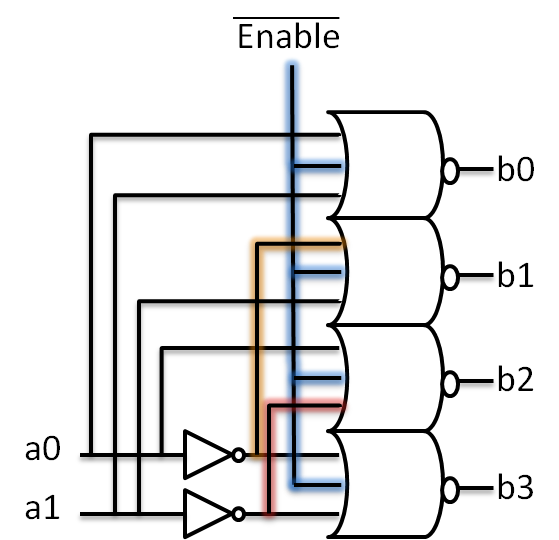
\includegraphics[width=0.5\textwidth] {../fig/hfdst-decoders-2to4.png} \label{fig:decoder2to4}}
\subfloat[3 naar 8 decoder]{ 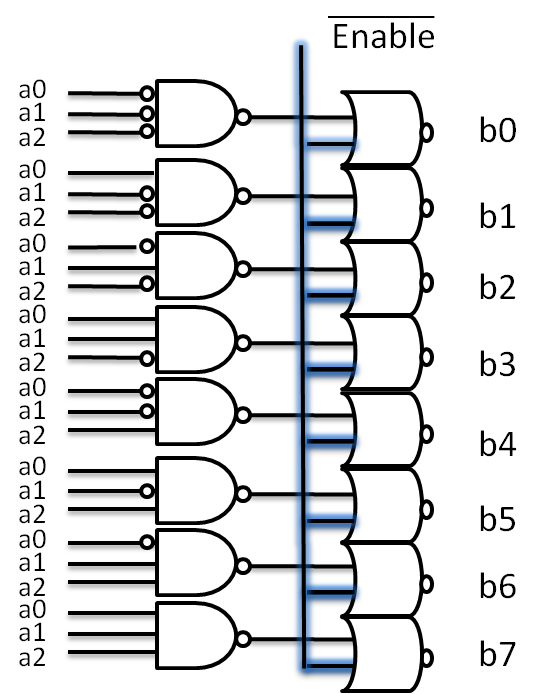
\includegraphics[width=0.5\textwidth] {../fig/hfdst-decoders-3to8.png} \label{fig:decoder3to8}}
\caption{basis decoders}
\end{figure}

\subsection{De grid decoder}
De grid decoder heeft een tweelaagse structuur. De eerste laag bestaat uit een aantal 2 naar 4 en/of 3 naar 8 decoders die in parallel staan. De verschillende uitgangen van deze eerste laag worden dan met AND-gates samen gevoed in een tweede laag. Om glitches te voor komen is het belangrijk dat al de signalen gelijktijdig binnen komen in de AND-gates, vandaar dat de architectuur van 2 naar 4 decoder van figure \ref{fig:decoder2to4} verandered werd tot een AND-OR architectuur zoals de architectuur van de 3 naar 8 decoder. Om de fanout tussen de eerste en tweede laag aan te kunnen, worden de AND-gates van de tweede laag geimplementeerd als OR gates met inverters aan de ingangen. Deze invertors werden dan afhankelijk van de fanout als buffers gesized. Tabel \ref{tab:griddecoder} geeft tenslotte weer hoe veel basis decoders er in de eerste laag van de grid decoder zitten en hoeveel and gates er in de tweede laag zitten, in functie van het aantal inputs

\begin{table}
\begin{center}
\begin{tabular}{llll}
\hline
\# inputs decoder & \# 2naar4 decoders & \# 3naar8 decoders & \# AND-gates\\
\hline
4 & 2 & 0 & 16\\
5 & 1 & 1 & 32\\
6 & 0 & 2 & 64\\
7 & 2 & 1 & 128\\
8 & 1 & 2 & 256\\
9 & 0 & 3 & 512\\
\hline
\end{tabular}
\end{center}
\caption{De verschillende aantal gates in de grid decoder}
\label{tab:griddecoder}
\end{table}

\subsection{Vergelijkende studie}
Eens ontworpen, kunnen de tree en grid decoders met elkaar vergelijken worden. Naast de gebruikelijke oppervlakte, energie en delay worden ook glitches, mismatch en delay verschill tussen verschillende addressen onderzocht. \\
Zoals in figuur \ref{fig:decoder_a} gezien kan worden, scaalt het oppervlakte van de grid decoder veel minder als die van de tree decoder bij een groter aantal inputs. De plotse stijging in het oppervalke van de tree decoder met 8 inputs kan verklaart worden door het gebruik van een extra laag in de boom structuur. \\
Het energie verbruik wordt vergeleken in figuur \ref{fig:decoder_ed}. De grid decoder heeft een lichte stijging van het energie verbruik infunctie van het aantal inputs, dit kan verklaart worden door het aantal gates dat geswitched wordt maar licht stijgt met het aantal inputs, daar naast gaat het meerste van de energie naar de buffers die de tweede laag aansturen (zie figuur \ref{fig:decoder_egrid}). De tree decoder aan de andere hand heeft een sterkere stijging van energie verbruik. dit kan verklaart worden door dat alle decoders in de tree architectuur gedeeltelijk switchen. Dit zou vermindered kunnen worden door de architectuur van de basis decoders (figuur \ref{fig:basisdecoders}) te veranderen zodat de enable vooraan komt te staan.\\
De delay van de decoders kan ook afgelezen worden in figuur \ref{fig:decoder_ed}. Beide decoders hebben ongeveer de zelfde delay. bij grote grid decoders kan de extra delay verklaart worden door het aansturen van een grote fanout.\\
Verder werden het opduiken van glitches onderzocht. In beide decoders is er de mogelijkheid dat er glitches op duiken. Het probleem bij deze decoders is het gebuik van de NOR-gates, de glitch duikt op als de ingang verandered van een 01 naar een 10 (zie figuur \ref{fig:decoder_glitch}) en er is een vertraging bij een van de twee ingangen. Bij de tree decoder duiken zijn deze glitches ingebaken in de architectuur aangezien de enable van een stage aangestuurt wordt door de vorige stage en hier altijd een zekere vertraging is. Bij de grid decoder daarentegen kan er glitch opduiken als de buffers die de tweede laag aansturen een asymetische delay hebben. Dit kan voor komen bij bv een 5 naar 32 decoder. de uitgangen van de 2naar 4 decoder en de 3 naar 8 decoder die hier in zitten zien een andere last. Deze buffers werden met zorg ontworpen om een asymetrische delay te voor komen.\\
Na een snelle mismatch analyse bleek dat de grid decoder minder variatie toon in energie verbruik en delay als de tree decoder. Tenslotte heeft de tree decoder grotere verschillen in delay, afhankelijk van welk het vorige en huidige address van de decoder is. Dit ziet men minder in de grid decoder. \\
Na het vergelijken van beide decoders op het vlak van oppervalkte, energie, delay, glitches, mismatch en delay verschil, Komt de grid decoder er als het beste uit en deze zal dan ook gebruikt worden in het finale ontwerp.


\begin{figure}[!ht]
\centering
\subfloat[oppervlakte]{ 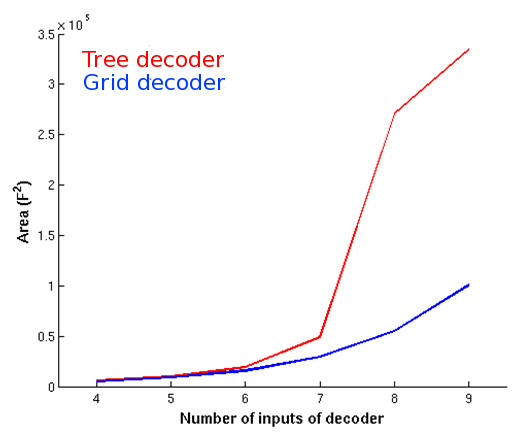
\includegraphics[width=0.5\textwidth] {../fig/hfdst-decoders-a.png} \label{fig:decoder_a}}
\subfloat[energie en delay]{ 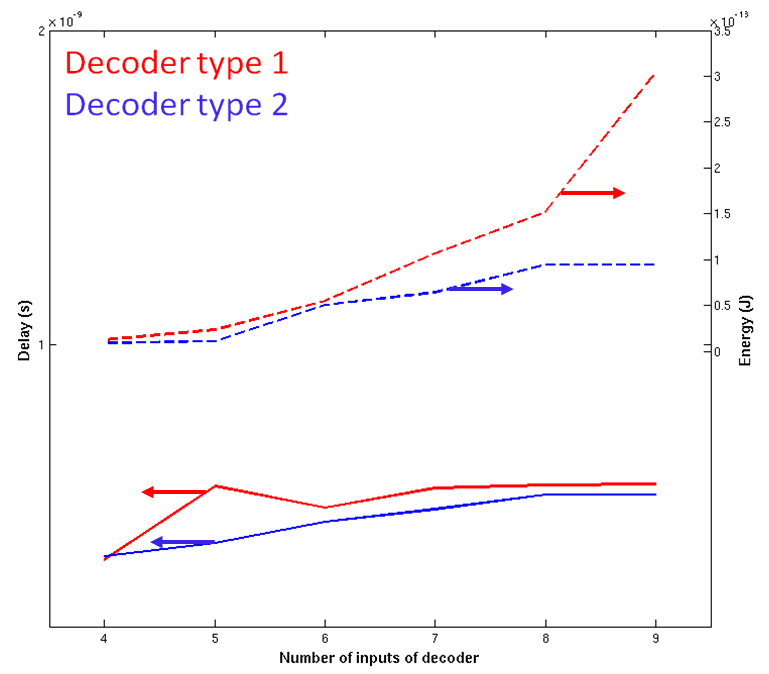
\includegraphics[width=0.5\textwidth] {../fig/hfdst-decoders-ed.png} \label{fig:decoder_ed}}
\caption{vergelijking van decoder types}
\end{figure}


\begin{figure}[!ht]
  \centering
  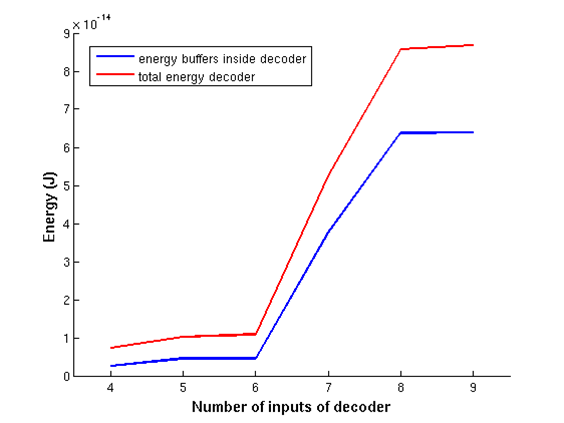
\includegraphics[width=0.8\textwidth]{../fig/hfdst-decoders-egrid.png}
  \caption{Energie verbruik in griddecoder}
  \label{fig:decoder_egrid}
\end{figure}

\begin{figure}[!ht]
  \centering
  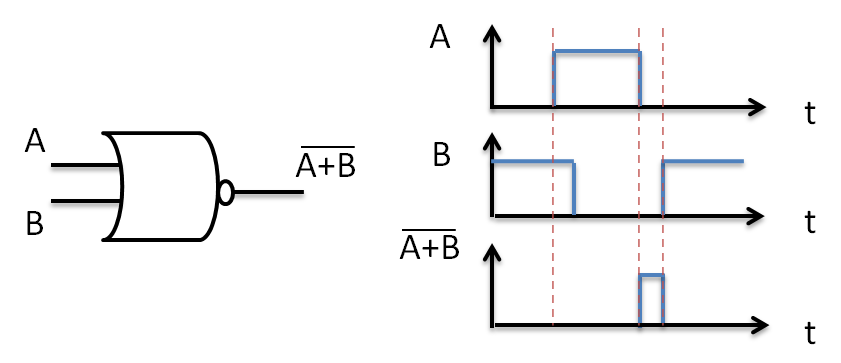
\includegraphics[width=0.8\textwidth]{../fig/hfdst-decoders-glitch.png}
  \caption{Glitch in NOR-gate}
  \label{fig:decoder_glitch}
\end{figure}


\section{Buffers}
Een digitale buffer is een logische component dat de uitgang van een andere logische block meer drijf kracht geeft om een grotere last sneller aan te sturen. Buffers worden op drie plaatsen in de geheugen architectuur gebruikt. Ten eerste om de woordlijnen aan te sturen. Ten tweede om de referentie logica aan te sturen en ten slotte  tussen de eerste en tweede laag in de grid decoders. Tabel \ref{tab:buffer} geeft een overzicht van het type last en het aantal lasten dat de verschillende buffers moeten aansturen.\\
De buffers werden ontworpen met logical effort waarbij het aantal stages en de sizing van elke stage werd bepaalt volgens het volgende stappen plan:
\begin{enumerate}
\item Bepaal de Path effort $F = GH$ waarbij $G = 1$ aangezien we enkel met inverters werken en $H = \frac{C_{out}}{C_{in}}$
\item Het aantal stages wordt bepaalt door $\hat{N} = log_{4}F$. hier bij werd er voor een stage effort van 4 gekozen voor een optimale delay \cite{Sutherland:1999:LED:298513}. \^{N} wordt dan afgerond tot een even getal N voor de woordlijn en referentie buffers, en tot een oneven getal voor de decoder buffers.
\item N wordt dan gebruikt om een nieuw stage effort \^{f} te berekenenn met de formule $\hat{f} = F^{1/N}$.
\item Ten slotte kunnen de de grotes van de verschillende invertoren in de chain berekend worden met de nieuw stage effort $\hat{f} = gh$.
\end{enumerate}
Figuur \ref{fig:refbuffer} illusteert de ongebufferde en gebufferde signalen die naar de referentie logica gaan, voor een verschillende aantal paralle geplaatste referentie logic.

\begin{table}
\begin{center}
\begin{tabular}{ccc}
\hline
 & Type Last & \# lasten\\
\hline
Woordlijn Buffer & 1 Transistor &  \#BL\\
Referentie Buffer & 1 Nor + 1 Inv &  \#BL\\
Decoder buffer & 1 Nor & 4 - 64\\
\hline
\end{tabular}
\end{center}
\caption{Lasten in de verschillende buffers}
\label{tab:buffer}
\end{table}

\begin{figure}[!ht]
  \centering
  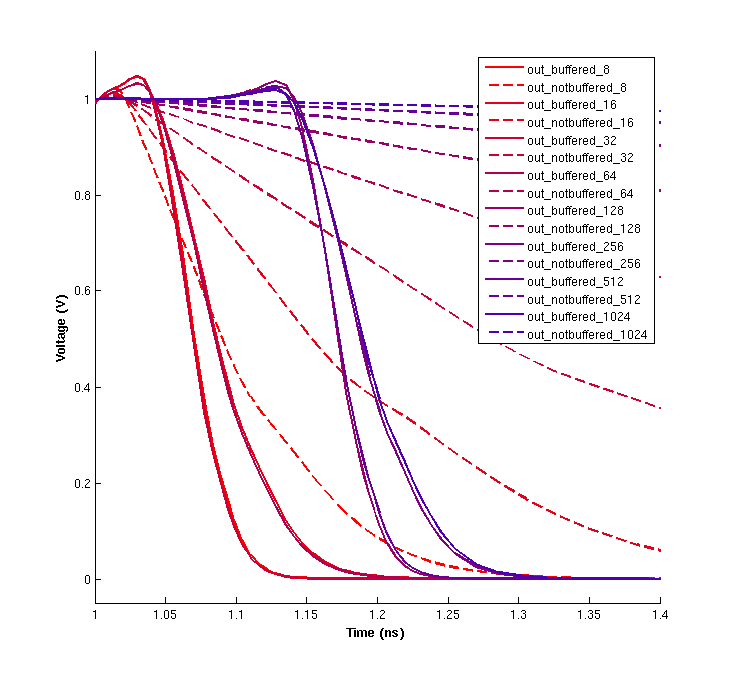
\includegraphics[width=0.8\textwidth]{../fig/hfdst-buffers-refbuffer.png}
  \caption{Gebufferde en ongebufferde signalen naar de referentie logica}
  \label{fig:refbuffer}
\end{figure}

\section{BL- en WL-drivers}

\section{Passgates}
Passgates zijn schakelaars die de spanning van een laagimpedant knooppunt doorlaten naar een hoogimpedant knooppunt. Idealiter heeft de passgate geen weerstand wanneer hij aanstaat. In de praktijk zal er altijd een beetje weerstand zijn, dit heeft als gevolg dat er een kleine RC-delay vooraleer het hoogimpedante punt is geladen/ontladen tot de waarde van het laagimpedante punt.
Een passgate kan gerealiseerd worden met een nMOS transistor, een pMOS of een combinatie van beiden.
In wat volgt worden de verschillende scenario's besproken die kunnen optreden wanneer de schakelaar aangezet wordt, de passgate zal immers niet altijd stroom kunnen leveren om het hoogimpedante knooppunt te (ont)laden.

\subsection{nMOS passgate}
De opstelling is het circuit van figuur \ref{fig:passgate1}. Afhankelijk van de (initiële) waardes van Vx en Vs, kunnen volgende situaties optreden.

\begin{figure}[h!]
  \centering
  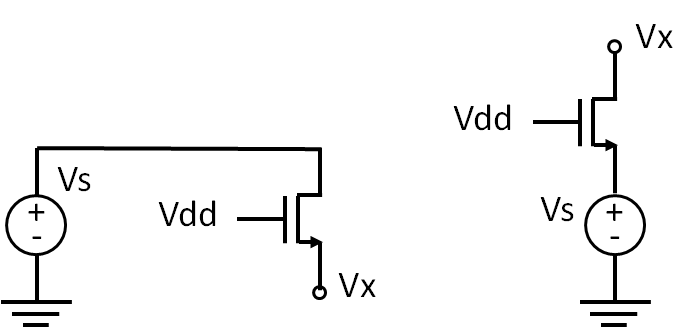
\includegraphics[width=0.5\textwidth]{../fig/hfdst-periphery-passgate1.png}
  \caption{nMOS passgate opstelling. a: Vs > Vx, b: Vs < Vx}
  \label{fig:passgate1}
\end{figure}

\begin{itemize}
\item Vx > Vs en Vdd - Vs > Vtn: de transistor gaat Vx ontladen tot Vs.
\item Vx > Vs en Vdd - Vs < Vtn: de transistor staat af, er gebeurt niets.
\item Vx < Vs en Vs < Vdd - Vtn: de transistor levert stroom tot Vx is opgeladen tot Vs.
\item Vx < Vs, Vs > Vdd - Vtn en Vx < Vdd - Vtn: de transistor gaat Vx opladen tot Vdd - Vtn.
\item Vx < Vs, Vs > Vdd - Vtn en Vx > Vdd - Vtn: de transistor staat af, er gebeurt niets.
\end{itemize}

\subsection{pMOS passgate}
De opstelling is het circuit van figuur \ref{fig:passgate2}. Er kunnen wederom verschillende situaties optreden.

\begin{figure}[h!]
  \centering
  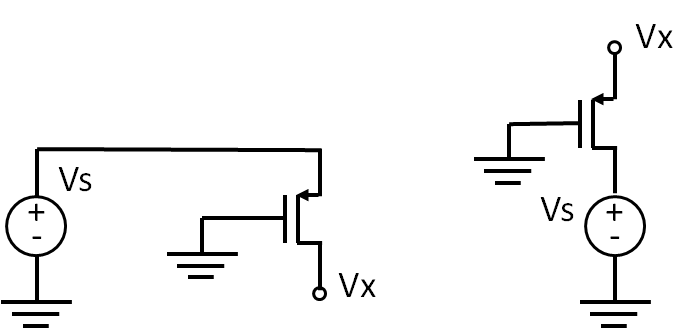
\includegraphics[width=0.5\textwidth]{../fig/hfdst-periphery-passgate2.png}
  \caption{pMOS passgate opstelling. a: Vs > Vx, b: Vs < Vx}
  \label{fig:passgate2}
\end{figure}

\begin{itemize}
\item Vs > Vx en Vs > |Vtp|: de transistor gaat Vx opladen tot Vs.
\item Vs > Vx en Vs < |Vtp|: de transistor staat af, er gebeurt niets.
\item Vs < Vx en Vs > |Vtp|: de transistor levert stroom tot Vx is ontladen tot Vs.
\item Vs < Vx, Vs < |Vtn| en Vx > |Vtp|: de transistor gaat Vx ontladen tot |Vtp|.
\item Vs < Vx, Vs < |Vtn| en Vx < |Vtn|: de transistor staat af, er gebeurt niets.
\end{itemize}

Er zijn dus spanningszones waarvoor de passgate niet functioneert, het is belangrijk te weten wat deze zones zijn, zodat het circuit ontworpen wordt om deze zones te vermijden. 
Op figuur \ref{fig:passgate3} worden deze zones in kaart gebracht voor een nMOS, een pMOS en een complementaire passgate, zowel voor LVT als HVT transistoren. Er dient opgemerkt te worden dat de passgates niet (of slechts even) aanstaan voor sommige zones, maar dat de uiteindelijke fout nog meevalt.
Als Vs bijvoorbeeld 0,9V bedraagt voor een nMOS passgate en Vx initieel 0,85V (met Vdd 1V), gaat de transistor geen stroom leveren, maar bedraagt de uiteindelijke fout 'slechts' 50mV.
In deze fout zit nog geen ladingsinjectie inbegrepen, eenmaal de passgate afschakelt is de injectie onvermijdelijk.
Zowel de LVT als de HVT complementaire passgates vertonen geen dode zones. Voor performantieredenen is geopteerd voor de LVT transistoren in het geheugenontwerp.

\begin{figure}[!ht]
\centering
\subfloat[CLVT]{ 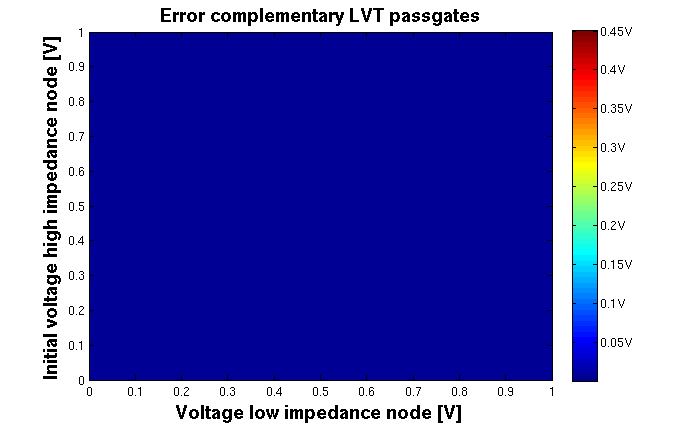
\includegraphics[width=0.5\textwidth] {../fig/hfdstk-periphery-CLVT.png}}
\subfloat[CHVT]{ 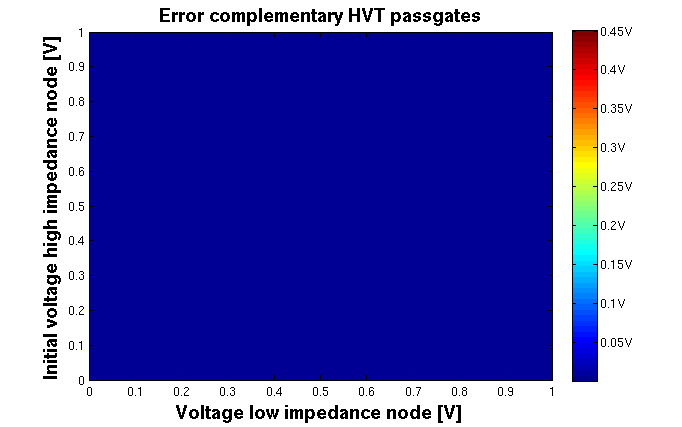
\includegraphics[width=0.5\textwidth] {../fig/hfdstk-periphery-CHVT.png}}\\
\subfloat[NLVT]{ 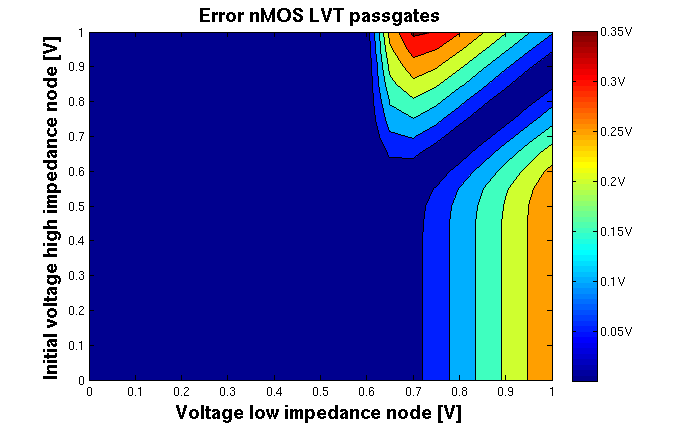
\includegraphics[width=0.5\textwidth] {../fig/hfdstk-periphery-NLVT.png}}
\subfloat[NHVT]{ 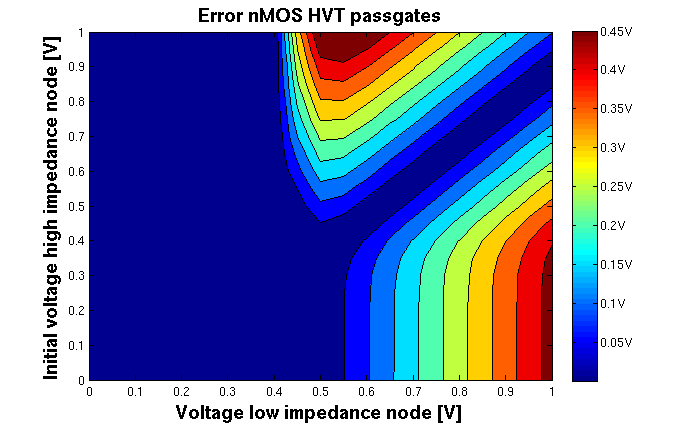
\includegraphics[width=0.5\textwidth] {../fig/hfdstk-periphery-NHVT.png}}\\
\subfloat[PLVT]{ 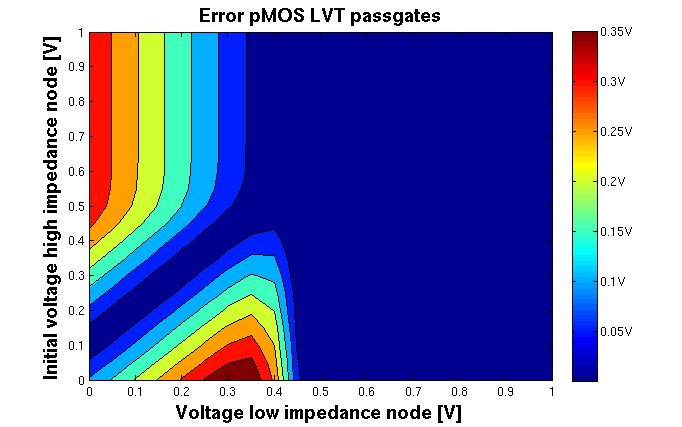
\includegraphics[width=0.5\textwidth] {../fig/hfdstk-periphery-PLVT.png}}
\subfloat[PHVT]{ 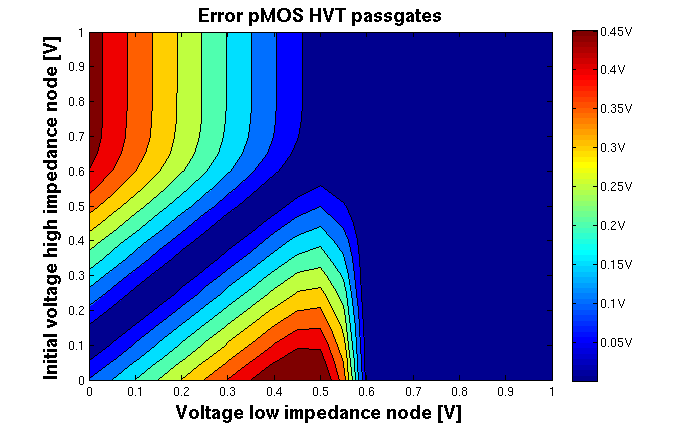
\includegraphics[width=0.5\textwidth] {../fig/hfdstk-periphery-PHVT.png}}
\caption{Dode zones voor verschillende types passgates}
\label{fig:passgate3}
\end{figure}



\section{Besluit}

